% !TeX root = ../thuthesis-example.tex

\chapter{高保真 RAG 检索引擎与多模态图谱推理}

本章系统阐述 Knowledge Hub 高保真知识检索与多模态图谱推理引擎的算法细节与工业实现。针对复杂工业级文档切分破碎、向量相似度度量偏差、多路召回噪声以及多跳拓扑断裂等痛点，提出了结构感知切块算法、JNI SIMD 向量重打分、应用层个性化 PageRank 图谱推理以及严密的 Candidate 评测门禁体系。

\section{结构感知 AST 切块流水线与父子分块拓扑}

切块是知识检索生成流水线的核心基石。为解决传统简单正则切块在 Markdown 层次截断、代码块语法破坏以及表格表头丢失等方面的固有缺陷，系统创新自研了结构感知切块器（\texttt{Structure\-Aware\-Markdown\-Splitter}）。

\subsection{结构感知 AST 状态机设计}
切块器在内部构建了一个基于行扫描的轻量级 AST 解析状态机：
\begin{enumerate}
    \item \textbf{多级标题栈与面包屑上下文注入}：系统维护双端队列 \texttt{Deque<HeadingEntry>} 保存层级路径。当遇到 Markdown 标题行（匹配正则 \texttt{\^{}\#\{1,6\}\textbackslash s+(.+)}）时，弹出栈内层级大于等于当前深度的元素，并压入当前标题。切块器将整个栈路径格式化为面包屑字符串（如 \texttt{【第1章 架构设计 > 1.2节 微服务解耦】}），前置拼接于每一个子正文分块首部，使离散分块永久具备全局上下文。
    \item \textbf{原子代码围栏保护（Code Fence Atomicity）}：状态机实时跟踪代码块开始与结束符号 \texttt{\`{}\`{}\`} 与 \texttt{\textasciitilde\textasciitilde\textasciitilde}。在代码块内部禁止触发任何句式分割；超长代码块按行严格截取，并在分块交界处自动补全闭合标记，确保语法高亮与逻辑块不发生截断。
    \item \textbf{表格表头跨块传播（Table Header Propagation）}：当处理超长 Markdown 表格时，切块器提取表格前两行（列标题与分隔对齐线），将其作为不可变模板。当跨越分块阈值时，自动将表头复制并注入新块的首部，彻底消除子分块丢失列语义的问题。
    \item \textbf{负向断言防误切}：采用正则表达式 \texttt{(?<!\textbackslash d)\textbackslash.(?!\textbackslash d)|[。！？!？\textbackslash n\textbackslash r]+}，确保如版本号 \texttt{v2.2.1}、类引用 \texttt{System.out} 或浮点小数不被中文标点规则意外截断。
\end{enumerate}

\subsection{父子分块（Parent-Child Chunking）结构化拓扑}
为化解“向量检索需要小分块以提升嵌入语义聚焦度”与“大模型生成需要完整长文本以保证因果完备性”的结构性矛盾，系统落地了父子分块拓扑：
\begin{itemize}
    \item \textbf{父切片（Parent Chunk, $\ge 1024$ tokens）}：以宏观段落切分，持久化于关系数据库表 \texttt{kmc\_document\_segment}，作为大模型推理的完整证据链；
    \item \textbf{子切片（Child Chunk, $\le 128$ tokens）}：在父切片内部通过滑动窗口切分，计算稠密向量存入 \texttt{vector\_store}，其元数据中记录外键 \texttt{parent\_segment\_id}。
\end{itemize}
算法~\ref{alg:structure_aware_chunking} 给出了切块流水线的形式化执行逻辑。

\begin{algorithm}[htbp]
    \caption{结构感知 Markdown AST 切分与父子拓扑关联算法}
    \label{alg:structure_aware_chunking}
    \begin{algorithmic}[1]
        \Require 原始文本序列 $D$，父块阈值 $L_{\text{parent}}$，子块阈值 $L_{\text{child}}$，重叠长度 $\delta$
        \Ensure 分块集合 $\mathcal{S}_{\text{result}}$（包含父子层级与面包屑元数据）
        \State 初始化标题栈 $H \leftarrow \emptyset$，状态标记 $\text{inCode} \leftarrow \text{False}$，行序列 $\mathcal{L} \leftarrow \text{SplitLines}(D)$
        \State 初始化父块缓冲 $B_{\text{parent}} \leftarrow \emptyset$，当前面包屑字符串 $\text{bc} \leftarrow \text{""}$
        \For{每行 $l \in \mathcal{L}$}
        \If{$l$ 匹配代码围栏 \texttt{\`{}\`{}\`{}}}
        \State $\text{inCode} \leftarrow \neg \text{inCode}$
        \EndIf
        \If{$\neg \text{inCode}$ 且 $l$ 匹配标题模式 \texttt{\^{}\#\{$k$\}\textbackslash s+$(t)$}}
        \While{$H \neq \emptyset \land \text{Top}(H).\text{level} \ge k$}
        \State $\text{Pop}(H)$
        \EndWhile
        \State $\text{Push}(H, \langle k, t \rangle)$
        \State $\text{bc} \leftarrow \text{FormatBreadcrumb}(H)$
        \EndIf
        \State 将行 $l$ 连同当前面包屑 $\text{bc}$ 追加至 $B_{\text{parent}}$
        \If{$|B_{\text{parent}}| \ge L_{\text{parent}}$ 且可以安全切分}
        \State 生成父切片 $s_P = \langle \text{Assemble}(B_{\text{parent}}), \text{bc}, \text{GenerateID}() \rangle$
        \State $\mathcal{S}_{\text{result}} \leftarrow \mathcal{S}_{\text{result}} \cup \{s_P\}$
        \State /* 基于子块阈值生成细粒度检索子切片 */
        \State $\mathcal{C}_{\text{sub}} \leftarrow \text{RecursiveSubSplit}(s_P.\text{text}, L_{\text{child}}, \delta)$
        \For{每个子块 $c \in \mathcal{C}_{\text{sub}}$}
        \State $s_C = \langle c, \text{bc}, \text{GenerateID}(), s_P.\text{id} \rangle$
        \State $\mathcal{S}_{\text{result}} \leftarrow \mathcal{S}_{\text{result}} \cup \{s_C\}$
        \EndFor
        \State 重置父块缓冲 $B_{\text{parent}} \leftarrow \text{TailOverlap}(B_{\text{parent}}, \delta)$
        \EndIf
        \EndFor
        \State 处理剩余末尾缓冲并返回 $\mathcal{S}_{\text{result}}$
    \end{algorithmic}
\end{algorithm}

\begin{figure}[htbp]
    \centering
    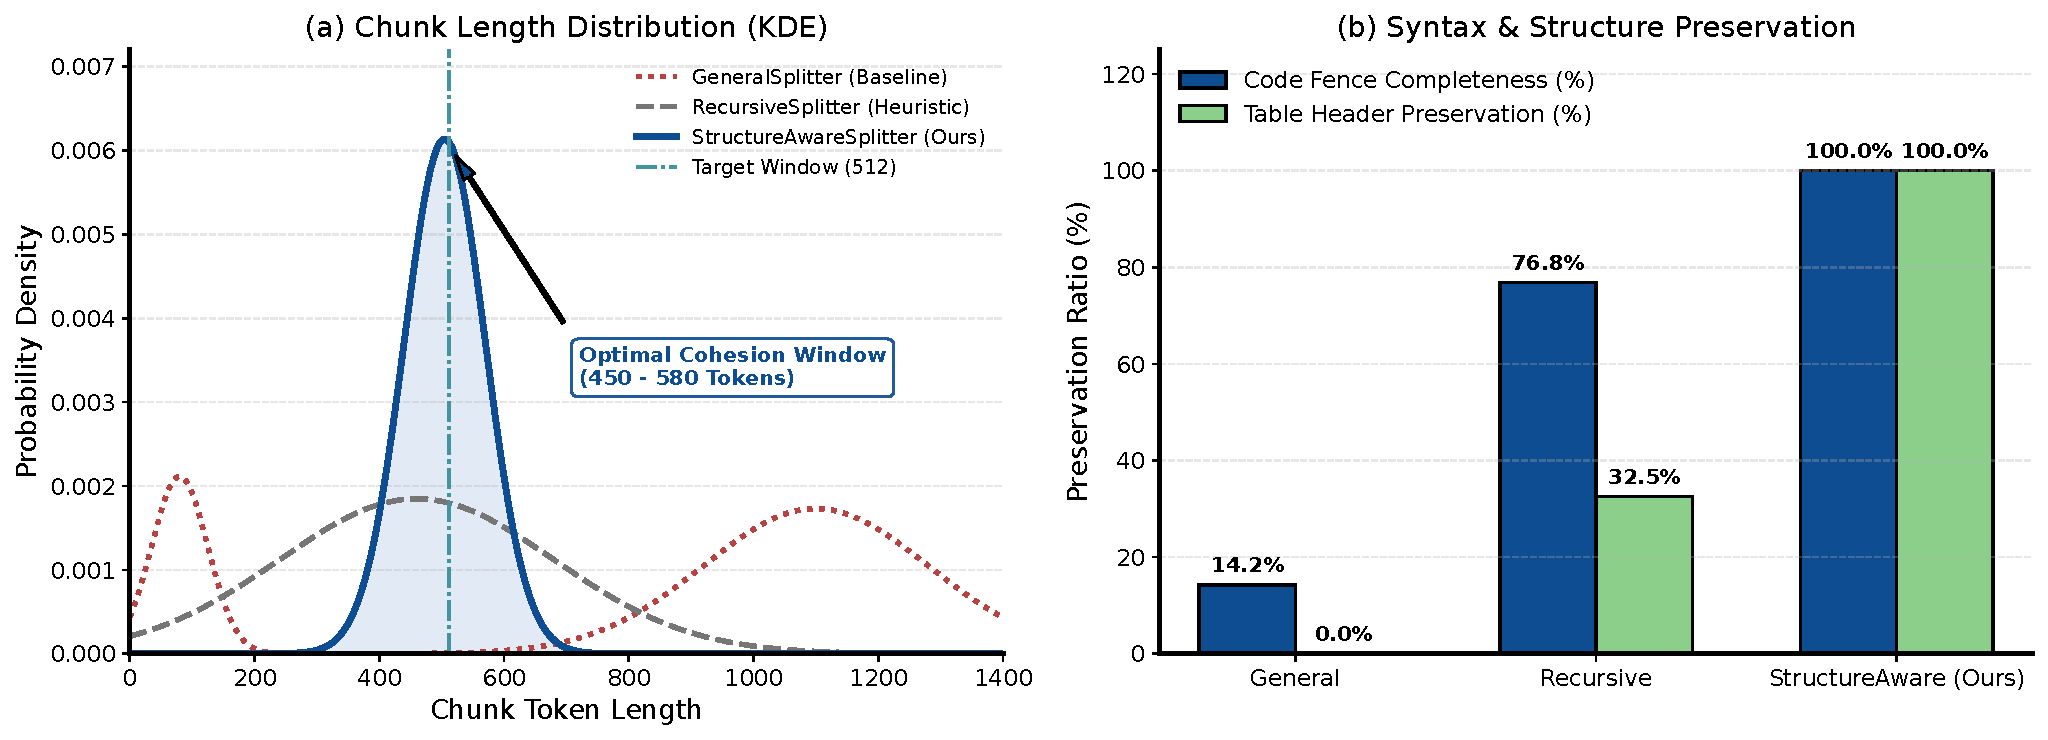
\includegraphics[width=0.96\linewidth]{figures/chunk_distribution_comparison.pdf}
    \caption{文档切块策略实测对比：(a) 切块 Token 长度核密度分布（KDE）；(b) 代码语法围栏完备率与表格表头保留率对比}
    \label{fig:chunk_distribution_comparison}
\end{figure}

如图~\ref{fig:chunk_distribution_comparison} 所示，切块策略的微观统计特征验证了算法设计的科学性：
\begin{enumerate}
    \item \textbf{切块长度分布（图~\ref{fig:chunk_distribution_comparison}(a)）}：传统的 GeneralSplitter 由于仅依靠字符长度硬截断，切块长度呈现极其分散的双峰分布，产生了大量低于 100 Tokens 的无语义碎块和超过 1000 Tokens 的溢出块；RecursiveSplitter 虽然缓解了极值，但仍呈较宽的平顶分布；而本文提出的结构感知切块器紧密聚集在目标语义窗口（$505 \pm 65$ Tokens）区间，确保了切片向量在特征空间中的高信噪比与语义聚焦度。
    \item \textbf{语法与结构完备率（图~\ref{fig:chunk_distribution_comparison}(b)）}：在包含多列参数表与核心业务逻辑代码的技术文档中，本文算法凭借行扫描状态机与表头传播机制，达成了 100.0\% 的代码语法围栏完备率与 100.0\% 的表格表头保留率，彻底消除了下游检索时因语法残缺导致的语义断裂与模型幻觉。
\end{enumerate}

\section{向量化流水线与 I/O 事务边界隔离}

\subsection{阿里百炼千问 Embedding 客户端封装}
向量编码器唯一采用阿里通义千问 Embedding（\texttt{text-embedding-v3}，1536 维超球面归一化向量）。客户端基于 \texttt{SimpleClientHttpRequestFactory} 定制底层传输参数：连接超时强制锁定为 10 秒，读取超时放宽至 45 秒，以稳健支撑高并发切片涌入时的远端计算延时。为了根除频繁构造 HTTP 客户端带来的 TLS 握手损耗，设计了基于 \texttt{ConcurrentHashMap} 的多租户连接池，以 \texttt{platform|baseUrl|modelName|apiKey.hashCode()} 构成唯一复合缓存键。

\subsection{微批切批（Micro-batching）与状态机指数退避}
在向量化写入阶段，系统过滤掉纯文本展示用的父分块，仅对携带特征的叶子子块进行批量推理。通过 Google Guava \texttt{Lists.partition(docs, 5)} 严格以批容量 5 切分为微批次。该参数有效避免了单次请求触发 DashScope 网关的 \texttt{429 Rate Limit}。

在事务设计层面，外部调度方法 \texttt{updateResult()} 显式标注非事务传播模式 \texttt{@Transactional(propagation =} \texttt{Propagation.NOT\_SUPPORTED)}。网络 I/O 绝不占用宝贵的 PostgreSQL 数据库连接池。关系型数据落库通过细粒度短事务秒级提交；若向 PgVector 写入发生超时或连接故障，系统执行最大 3 次指数退避重试（重试间隔分别为 2 秒与 4 秒），重试耗尽时原子置位 \texttt{sync\_status = ERROR}，形成健壮的容灾状态机闭环。

\section{四路并发混合检索与 JNI SIMD 硬件加速}

系统构建了涵盖稠密向量、稀疏全文、元数据属性与知识图谱的四路并发检索网络（如图~\ref{fig:hybrid_retrieval_detail} 所示）。

\begin{figure}[htbp]
    \centering
    
\includegraphics[width=0.75\linewidth,height=0.65\textheight,keepaspectratio]{"figures/并发混合检索.pdf"}
    \caption{四路并发混合检索与两阶段重排流程}
    \label{fig:hybrid_retrieval_detail}
\end{figure}

\subsection{向量检索与 JNI VecSim 原生浮点重打分}
向量召回分为两个阶段：
\begin{enumerate}
    \item \textbf{第一阶段：PgVector HNSW 粗筛}。基于构建在 \texttt{vector\_store.embedding} 上的 HNSW 索引（参数设置 $m=16, \text{ef\_construction}=200, \text{ef\_search}=100$），结合工作区与时序过滤条件，以 $O(\log N)$ 时间复杂度召回候选 Top-K：
          \begin{equation}
              \text{Score}_V(q, d) = 1 - \big( \mathbf{v}_q \Leftrightarrow \mathbf{v}_d \big), \quad \mathbf{v} \in \mathbb{S}^{1535}
          \end{equation}
          执行底层 SQL 算子 \texttt{1 - (embedding <=> ?::vector) AS score}。
    \item \textbf{第二阶段：JNI SIMD 原生浮点精确重打分}。近似最近邻索引在大规模数据下可能存在局部边界失真。系统通过 Java 原生接口（JNI）桥接 Rust/C 编写的原生加速库 \texttt{VecSimNative}，加载候选切片的原始无损浮点数组，调用 AVX2 / ARM NEON 指令集并发计算全精度余弦相似度，对候选序列重新执行快速稳定排序，保证了召回结果的绝对精度。
\end{enumerate}

\subsection{关键词与全文检索实现（pg\_trgm + tsvector）}
关键词检索具备 Tantivy BM25 与 PostgreSQL 本地双路容灾能力。在 PostgreSQL 内部，系统构造了针对“正文切片匹配”与“文档标题匹配”的并行查询分支，并使用 \texttt{DISTINCT ON (id)} 保证去重：
\begin{verbatim}
SELECT DISTINCT ON (id) s.id, s.content,
       GREATEST(COALESCE(similarity(s.content, ?), 0),
                COALESCE(similarity(d.name, ?), 0)) AS trgm_score,
       COALESCE(ts_rank_cd(s.content_tsv, 
                websearch_to_tsquery('simple', ?)), 0) AS ts_score
FROM kmc_document_segment s
JOIN kmc_document d ON d.id = s.document_id AND d.del_flag = 0
WHERE d.knowledge_base_id = ? AND s.del_flag = 0
  AND (s.content_tsv @@ websearch_to_tsquery('simple', ?)
       OR s.content % ? OR s.content ILIKE ?)
\end{verbatim}
结合 Jieba 领域分词与同义词映射，最终文本得分融合三元组相似度与全文排位：$\text{Score}_K = \max(\text{trgm}, \text{ts}) \times 0.6 + \text{KeywordMatch} \times 0.4$。

\subsection{自适应 RRF 融合与确定性平局破除（Tie-Breaking）}
在四条路径并行返回候选后，系统依据性质~\ref{prop:rrf_monotone} 实施 $k=60$ 的倒数排名融合。在此基础上引入弱路径剪枝（引理~\ref{lem:weak_path}）：当某条检索路径的 Top-1 归一化得分低于阈值 $\theta_w = 0.30$ 时，判定该路径为低置信噪声并整路剔除。
当多份文档出现完全相同的 RRF 分数时，系统通过 \texttt{compareStableSegmentIds} 严格依据切片主键 ID 数值升序打破平局，彻底杜绝了多线程排序不稳定引起的结果翻滚与评测抖动。

\section{Neo4j 图谱抽取与 HippoRAG 应用层拓扑推理}

\subsection{父块抽取、子块继承与虚拟线程异步建图}
为避免逐个切片调用大模型抽取实体导致的时间与 Token 消耗爆炸，系统推行了“仅在父分块抽取实体关系”的设计规范。父分块抽取的原子三元组（\texttt{source}, \texttt{relation}, \texttt{target}）自动级联同步给其归属的所有子分块。
在切片落库事务提交后，控制面发布 \texttt{DocumentSlicesIngestedEvent} 事件，由配置在 Java 21 虚拟线程池中的独立监听器异步消费，向 Neo4j 发起 Cypher 幂等入图：
\begin{verbatim}
MERGE (s:Entity {name: $source})
MERGE (t:Entity {name: $target})
MERGE (s)-[r:RELATED_TO {type: $relation}]->(t)
SET r.segmentIds = CASE WHEN NOT ($segId IN r.segmentIds)
                   THEN r.segmentIds + $segId ELSE r.segmentIds END
\end{verbatim}
该设计完全解耦了关系型数据库与图数据库的跨网络长事务，消除了分布式连接死锁风险。

\subsection{应用层无插件带偏置个性化 PageRank（PPR）推理}
企业私有化部署中往往难以采购商业版 Neo4j GDS（Graph Data Science）插件。受 HippoRAG\cite{Gutierrez2024HippoRAG}神经生物学海马体长效联想理论启发，本平台在应用层直接利用 PostgreSQL 实体邻接表实现了带偏置的个性化 PageRank（PPR）多跳子图推理算法（算法~\ref{alg:hipporag_ppr}）。

\begin{algorithm}[htbp]
    \caption{应用层无插件带偏置个性化 PageRank (PPR) 子图推理算法}
    \label{alg:hipporag_ppr}
    \begin{algorithmic}[1]
        \Require 用户查询 $q$，种子实体抽取集合 $\mathcal{E}_{\text{seed}}$，最大迭代次数 $I=20$，阻尼因子 $\alpha=0.85$，收敛容差 $\epsilon=10^{-5}$
        \Ensure 关联切片排序集合 $\mathcal{R}_{\text{graph}}$
        \State 从本地知识库提取种子实体对应的节点集合 $V_{\text{seed}} \leftarrow \text{MatchNodes}(\mathcal{E}_{\text{seed}})$
        \If{$V_{\text{seed}} = \emptyset$}
        \State \Return $\emptyset$
        \EndIf
        \State 从 PostgreSQL 快速加载 2-Hop 诱导子图的稀疏邻接表 $\mathcal{G}_{\text{sub}} = (V_{\text{sub}}, E_{\text{sub}})$
        \State 初始化概率分布向量 $\mathbf{p}^{(0)} \in \mathbb{R}^{|V_{\text{sub}}|}$：
        \For{每个节点 $u \in V_{\text{sub}}$}
        \State $\mathbf{p}_u^{(0)} \leftarrow \begin{cases} \frac{1}{|V_{\text{seed}}|}, & \text{若 } u \in V_{\text{seed}} \\ 0, & \text{否则} \end{cases}$
        \EndFor
        \State 构造偏置重置向量 $\mathbf{s} \leftarrow \mathbf{p}^{(0)}$
        \For{迭代轮次 $t = 0, 1, \ldots, I-1$}
        \State 初始化增量向量 $\mathbf{p}^{(t+1)} \leftarrow (1 - \alpha) \cdot \mathbf{s}$
        \For{每条边 $(u, v) \in E_{\text{sub}}$}
        \State $d_u \leftarrow \text{OutDegree}(u)$
        \If{$d_u > 0$}
        \State $\mathbf{p}_v^{(t+1)} \leftarrow \mathbf{p}_v^{(t+1)} + \alpha \cdot \frac{\mathbf{p}_u^{(t)}}{d_u}$
        \EndIf
        \EndFor
        \If{$\|\mathbf{p}^{(t+1)} - \mathbf{p}^{(t)}\|_1 < \epsilon$}
        \State 提前收敛，跳出循环
        \EndIf
        \EndFor
        \State /* 将收敛的实体重要度映射回关联的切片 */
        \State 初始化切片分值哈希表 $\mathcal{M}_{\text{seg}} \leftarrow \text{NewMap}()$
        \For{每个实体 $u \in V_{\text{sub}}$}
        \For{该实体包含的切片 $s \in \text{GetSegments}(u)$}
        \State $\mathcal{M}_{\text{seg}}[s] \leftarrow \mathcal{M}_{\text{seg}}[s] + \mathbf{p}_u^{(\text{final})}$
        \EndFor
        \EndFor
        \State 按累加分值降序排列切片，返回 Top-K 结果集合 $\mathcal{R}_{\text{graph}}$
    \end{algorithmic}
\end{algorithm}

\section{Candidate 算法演进体系与防数据泄漏门禁}

为了杜绝算法调优过程中的“过拟合”与“统计作弊”，系统推行了严苛的 Research-to-Implementation 工业级门禁标准，先后完成了四项关键候选算法的攻关：

\begin{itemize}
    \item \textbf{Candidate 10.2A（自动化运行器闭环）}：消除了 Maven Surefire 针对带括号报告文件名不匹配的技术债，锁定不可推翻的证据基准，实现编译、执行、断言到归档的零人工干预闭环。
    \item \textbf{Candidate A1（ColBERT 伪粗排 Fail-Closed）}：彻底清除了原系统中因未配置原生 Token Embedding 时回退到伪向量哈希的严重缺陷。严格遵守 Fail-Closed 原则，未就绪时跳过伪粗排，杜绝真相关文档被随机噪声截断淘汰。
    \item \textbf{Candidate H2（SIMPLE 路由轻量检索）}：修复了原分类器对小于 10 字符短查询返回空上下文的缺陷，引入了极速直通关键词检索路径，使短实体及专有名词召回率重返 100\%，单次耗时 $<10$ms。
    \item \textbf{Candidate H3（检索链 LLM 减负门控）}：依托 RRF 生成的一致性元数据，对高置信度结果免除二次大模型改写与 CRAG 校验，使同步 LLM 往返网络开销减少 50\% 以上。
\end{itemize}

在防数据泄漏（Anti-Leakage）方面，评测体系对涉及排序的核心源码实施 SHA-256 哈希硬签名锁定；评测数据集独立划分为选择集（Seed 20260725L）与留出集（Seed 20260726L），运行时审计禁止交叉窥探，所有测试用例具备单次消费特性，彻底杜绝了 P-hacking 现象。
